\part{A Matemática do Bitcoin}
\label{ch:capitulo4}
\chapter*{A Matemática do Bitcoin}

Antes de podermos discutir como a Prova de Trabalho é validada, precisaremos de uma introdução rápida em Ciência da Computação sobre dois conceitos: bits e criação de hash.

\paragraph{Criando um Hash}
\paragraph{}

O quebra-cabeça de Prova de Trabalho assimétrico do Bitcoin envolve o uso de uma função hash. Da álgebra básica, sabemos que uma função é uma caixa onde você \textit{insere} um valor de entrada \textit{x} e obtém um valor de saída \textit{f(x)}. Por exemplo, a função \textit{f(x)=2x} pega um valor e o multiplica por dois. Portanto, a entrada \textit{x=2} nos dá a \textit{saída f(x)=4}.

Uma função hash é uma função especial, onde você insere qualquer sequência de letras, números ou outros dados, como “Olá, mundo”, e obtém um número gigante que parece algo totalmente aleatório:

\begin{quote}{1111811713258219242661329357757490458455 \newline
4890446643616001126584346633541502095
}\end{quote}

A função hash particular usada acima na string "Hello, World" é chamada de sha256 e, por acaso, é a que o Bitcoin usa.

\begin{figure}
  \centering
  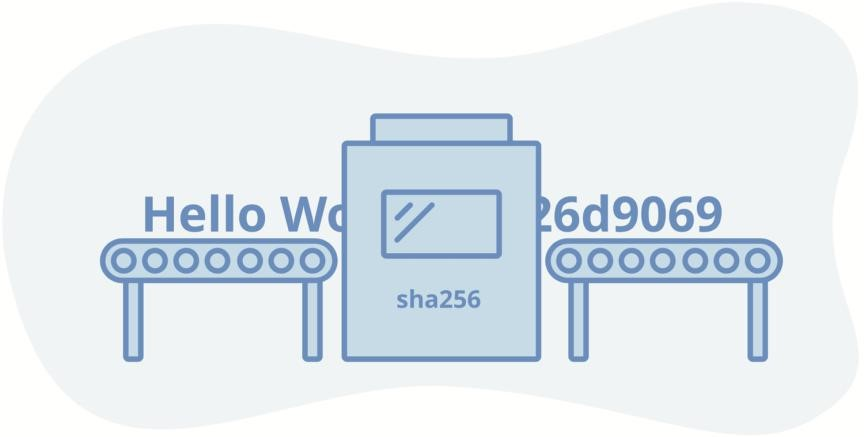
\includegraphics[width=10cm]{imagens/hash-capitulo-04.jpg}
  \caption{Fazendo o hash de uma string}
\end{figure}

A função hash sha256 tem as seguintes propriedades que são úteis para nós:

\begin{enumerate}
\item A saída é determinística: você sempre obtém a mesma saída para a mesma entrada;
\item A saída é imprevisível: alterar apenas uma letra ou adicionar um espaço à string de entrada mudará drasticamente a saída, tanto que você não pode encontrar nenhuma correlação com os dados de entrada original;
\item É rápido calcular o hash para dados de entrada de qualquer tamanho;
\item É impossível encontrar duas strings que geram hash para a mesma saída;
\item Dado o hash de saída de sha256, é impossível retornar à string de entrada. Chamamos isso de função unilateral;
\item A saída é sempre um tamanho específico (256 bits para sha256).
\end{enumerate}

\newpage

\paragraph{Uma introdução rápida sobre bits}
\paragraph{}

O sistema numérico que você conhece e adora, composto dos números de 0 a 9, é chamado de \textit{decimal} porque possui dez dígitos. Os computadores, por outro lado, preferem um sistema numérico diferente, feito de uns e zeros, indicando a presença ou ausência de um sinal elétrico. Este sistema numérico é chamado de \textit{binário}.

No sistema decimal, você usa apenas os dígitos de 0 a 9. Se você usar apenas um dígito, poderá representar dez números diferentes, de 0 a 9. Se usar dois dígitos, poderá representar 10x10=100 números diferentes: 00, 01,\ldots a 99. Para três dígitos, você pode ter 10x10x10=1000 números: 000, 001,\ldots a 999.

Espero que você esteja começando a ver um padrão. Para descobrir o tamanho de um número que podemos representar com N dígitos, multiplicamos dez por ele mesmo N vezes. Em outras palavras, \(10^N\), ou 10 elevado à potência de N.

O binário funciona da mesma maneira. A única coisa que muda é o número de dígitos que estão disponíveis para nós. Embora estejamos acostumados com decimais com dez dígitos, um \textit{dígito binário} ou \textit{bit} só pode ter dois valores: zero e um.

Se 1 bit pode representar dois valores, então dois bits podem representar 4 valores: 00, 01, 10, 11. Você pode calcular isso multiplicando 2x2, pois cada dígito pode ter dois valores.

Três bits podem representar 2 x 2 x 2 = \(2^3\) = 8 valores, que são 000, 001, 010, 011, 100, 101, 110, 111.

Portanto, um número \textit{binário} de N \textit{bits} pode ser representado como \(2^N\) valores diferentes.

Portanto, o número de valores exclusivos que você pode representar com 256 bits, o tamanho da função de hashing sha256, é \(2^{256}\). Esse é um número gigante, quase inconcebível para a mente humana. Representado em decimal, esse número tem 78 dígitos. Para colocar isso em perspectiva, isso é mais ou menos o número estimado de átomos em todo o universo conhecido.


\begin{multline}
\begin{aligned}
2^{256} = & 115.792.089.237.316.195.423.570.985.008.\\
& 687.907.853.269.984.665.640.564.039.457.\\
& 584.007.913.129.639.936
\end{aligned}
\end{multline}


Este é o número de saídas possíveis quando você faz o hash de qualquer string com a função de hash sha256. Portanto, é efetivamente impossível prever como será o número produzido por essa função. Seria como prever 256 jogadas de moeda em sequência ou adivinhar a localização de um átomo específico que escolhi em algum lugar do universo.

Este número é muito longo para continuar escrevendo, então diremos apenas \(2^{256}\) de agora em diante, mas espero que isso acione uma imagem mental de um universo de possibilidades para você.

\paragraph{Vamos transformar algumas strings em hash}
\paragraph{}

Aqui estão algumas strings de exemplo e seus hashes sha256. O resultado está em números decimais, embora dentro de um computador eles apareceriam como uma sequência binária de uns e zeros.

O objetivo aqui é demonstrar como o número muda drasticamente com base em uma pequena mudança na string de entrada. Você não pode prever a saída produzida pela função hash com base no que você colocou nela:

\begin{samepage}
\begin{quote}{"Hello World!"\newline
52740724284578854442640185928423074974\newline
81806529570658746454048816174655413720\newline
}\end{quote}
\end{samepage}

\begin{samepage}
\begin{quote}{"Hello World!!"\newline
958633198749395357316023441946434972583\newline
74513872780665335270495834770720452323\newline
}\end{quote}
\end{samepage}

Não há como ninguém, nem mesmo um computador, olhar para o número de aparência aleatória resultante e descobrir a string que o criou. Se você quiser brincar com o sha256, há alguns sites online onde você pode experimentar fazer o hash de qualquer informação que desejar. por exemplo \url{https://passwordsgenerator.net/sha256-hash-generator/}

\paragraph{Criando um hash para ganhar na loteria de prova de trabalho}
\paragraph{}
 

Tudo bem, agora estamos prontos para falar sobre a parte chave da magia. Dissemos que há \(2^{256}\) valores de saída de sha256 possíveis no total. Para tornar mais fácil de entender, vamos fingir que há apenas um total de 1000 saídas hash possíveis.

O nosso sistema de loteria funciona assim:

\begin{enumerate}
\item Ana anuncia que deseja enviar R\$2,00 para Bruno;
\item Todo mundo que quer tentar a sorte na loteria pega esta transação “Ana envia R\$2,00 para Bruno”, adicionando um número aleatório chamado \textit{nonce} (número usado apenas uma vez) no final. Isso é para ter certeza de que a string que eles estão fazendo o hash é diferente de qualquer outra pessoa, ajudando-os a encontrar um número vencedor na loteria;
\item Se esse número for menor do que o \textit{Número Alvo} (veremos isso em um segundo), eles ganham na loteria;
\item Se o número que eles obtiverem for maior do que o número alvo, eles tentam fazer o hash novamente, adicionando nonces aleatórios: “Ana envia R\$2,00 para Bruno com nonce = 12345”, “Ana envia R\$2,00 para Bruno com nonce = 92435”, “Ana envia R\$2,00 para Bruno nonce = 132849012348092134” e assim por diante, até que o número hash resultante seja menor que o \textit{Número Alvo}.
\end{enumerate}

Pode levar muitas, muitas tentativas para encontrar um hash que seja menor que o número alvo. Portanto, a ideia aqui é esta: se houver 1000 hashes possíveis e definirmos o número alvo como 100, qual porcentagem de hashes está abaixo do alvo?

Esta é a matemática básica: de 1000 números possíveis, de zero a 999, existem 100 números que são menores que 100 e 900 números que são maiores. Portanto, 100/1000 ou 10\% dos hashes são menores que o destino. Então, se você fizer um hash com qualquer string e sua função hash produzir 1000 saídas diferentes, você espera obter um hash abaixo do alvo limitado a 100, cerca de 10\% do tempo.

É assim que a loteria funciona: nós definimos um \textit{alvo} e todos concordamos com ele (falaremos sobre como isso funciona em breve). Então, pegamos as transações sobre as quais as pessoas estão nos contando e fazemos o hash, adicionando um nonce aleatório no final. Assim que alguém encontra um hash que está dentro do limite imposto pelo alvo, nós o anunciamos para todos na rede:

Olá pessoal:
\begin{itemize}
\item Peguei as transações: "Ana envia R\$2,00 para Bruno, Carol envia R\$5,00 para Ana";
\item Adicionei o nonce "32895";
\item O resultado foi um hash com retorno 42, que é menor que o alvo limite de 100;
\item Aqui está minha prova de trabalho: os dados da transação, o nonce que usei e o hash que foi produzido com base nessas entradas.
\end{itemize}

Para isso, talvez seja necessário bilhões de tentativas de hash para conseguir o resultado, gastando milhares de dólares em energia, mas todos podem imediatamente validar que fiz certo porque eles podem fazer o hash em uma única tentativa, já que dei a entrada e o saída esperada. Lembre-se de que os hashes são impossíveis de serem revertidos, mas são fáceis de serem calculados!

Como isso está ligado ao gasto de energia? Bem, já dissemos que o conjunto de todos os hashes possíveis é na verdade um número gigante que é quase tão grande quanto o número de átomos no universo. Agora podemos definir o \textit{alvo} como baixo para que apenas uma pequena fração dos hashes sejam válidos. Isso significa que qualquer pessoa que quiser encontrar um hash válido terá que gastar uma grande quantidade de tempo e processamento o que significa que terá que gastar eletricidade, para encontrar um número de hash menor que nosso alvo.

Quanto menor o alvo, mais tentativas serão necessárias para encontrar um número que funcione. Quanto maior o alvo, mais rápido podemos encontrar um hash vencedor.